\begin{figure*}[t]
    \centering
    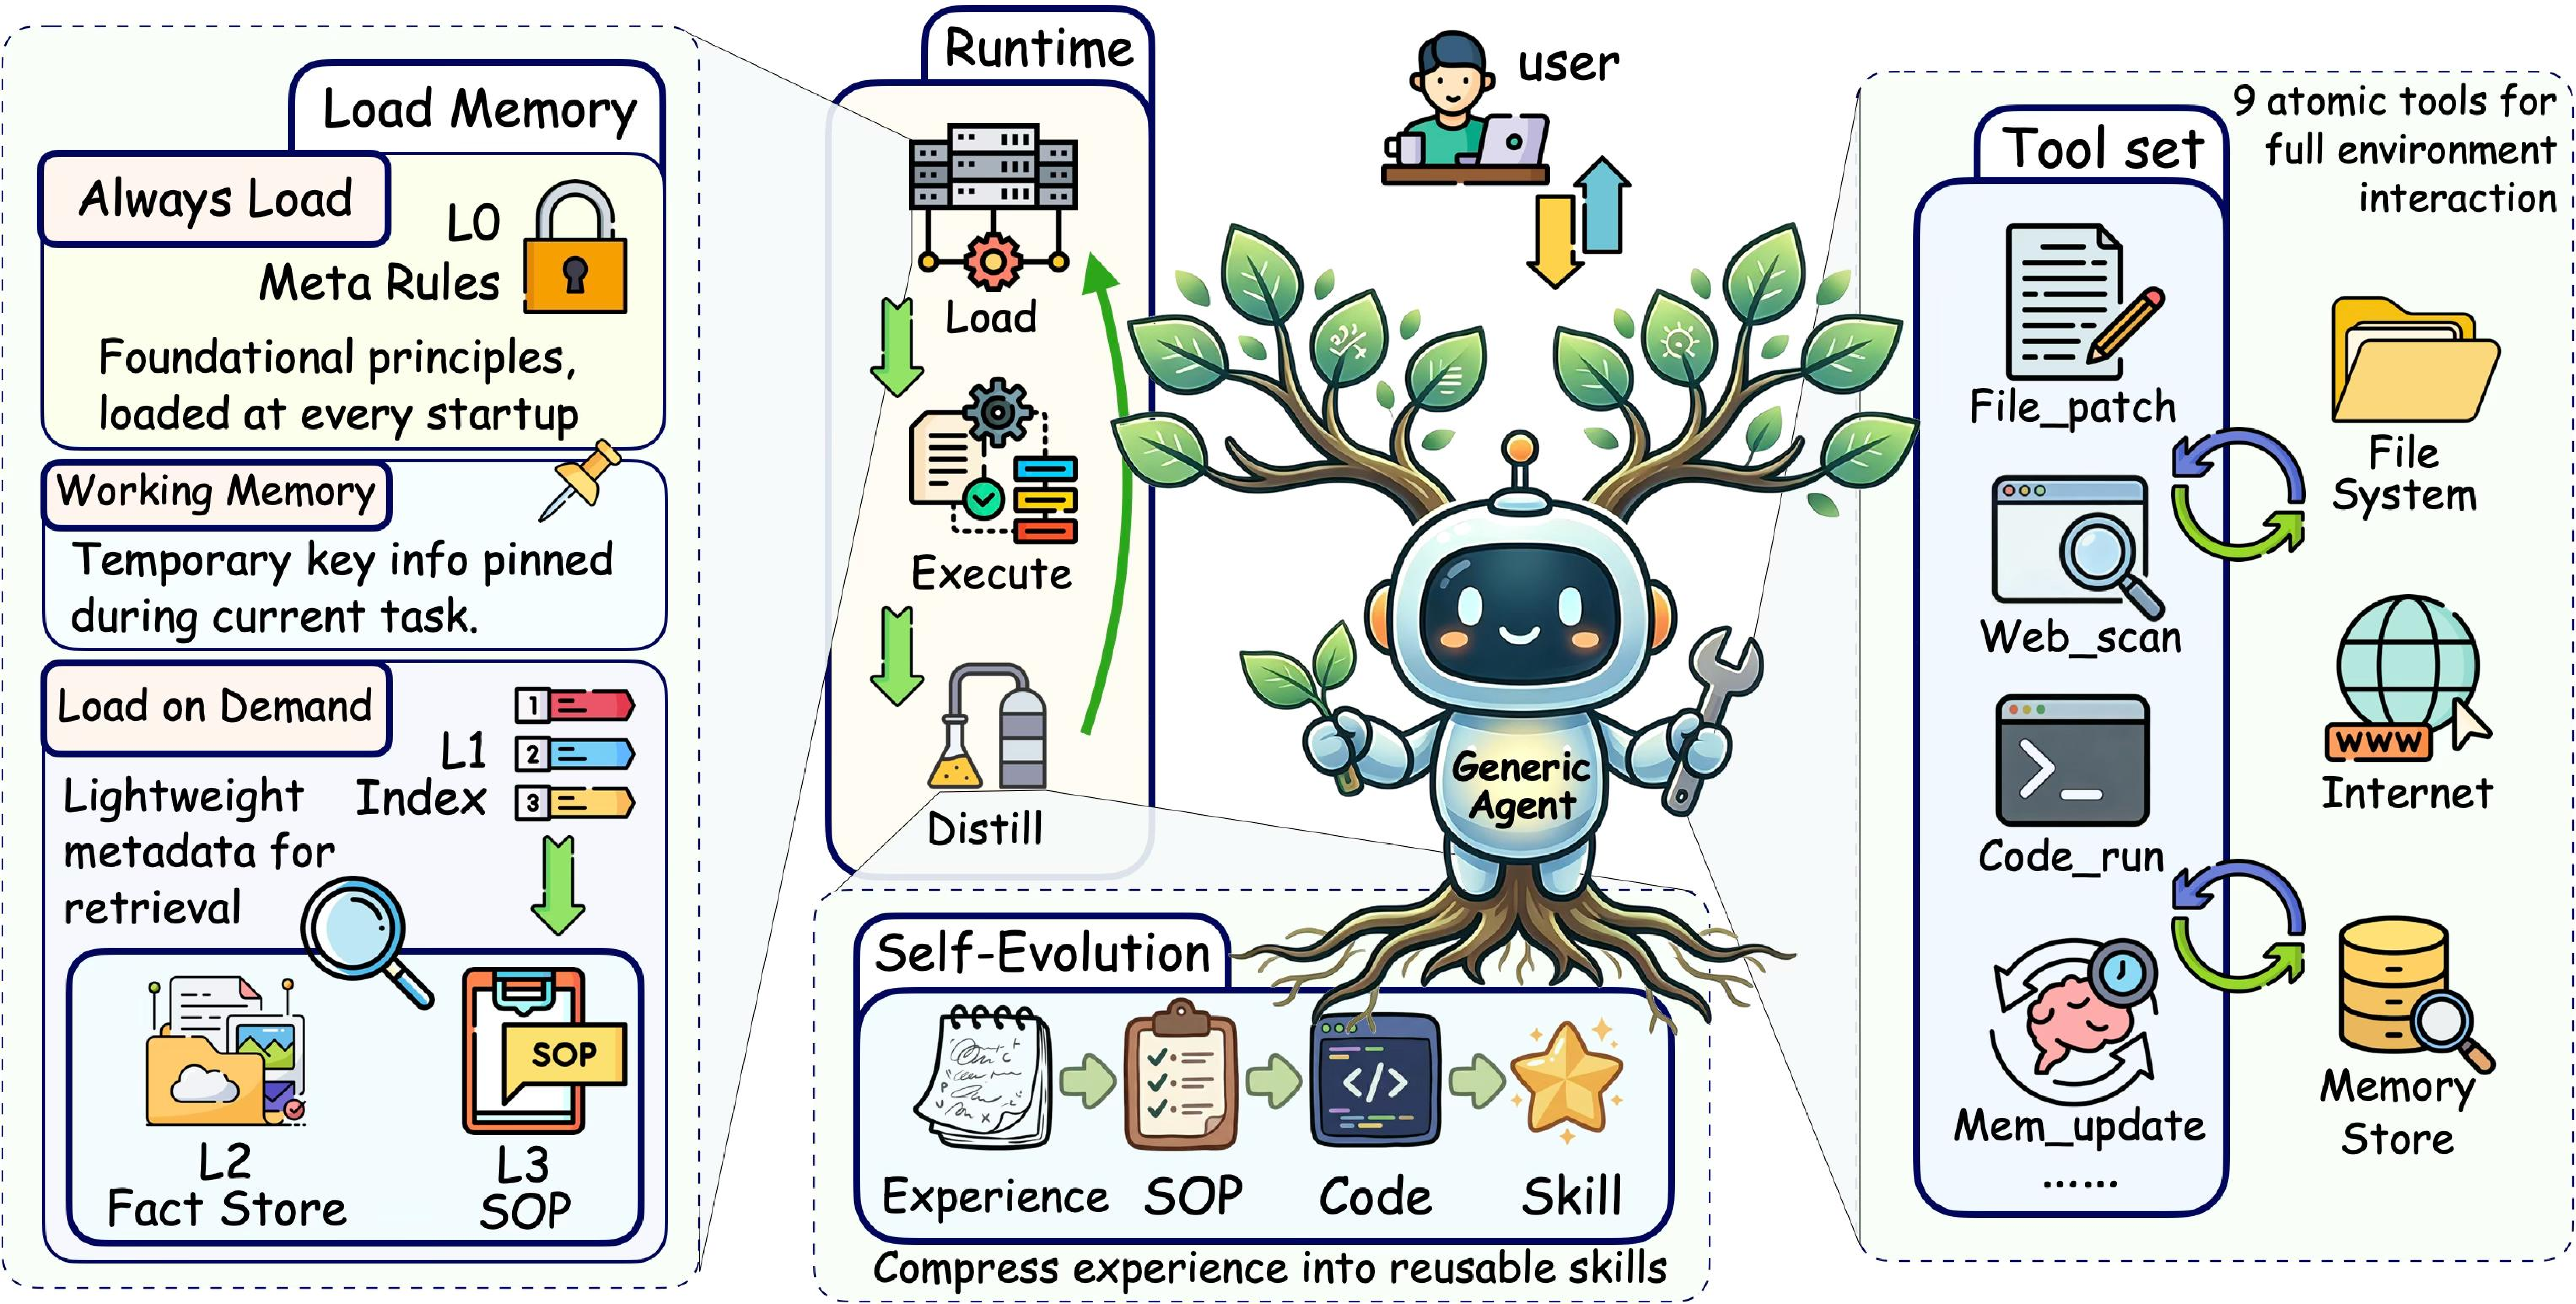
\includegraphics[width=0.98\linewidth]{image/framework_0413.pdf}
    \caption{\textbf{Overall framework of GA.}}
    \label{fig:agent_loop}
\end{figure*}

\subsection{Design Principles}
\label{sec:principle}
\begin{AIbox}
GA is designed around the principle of \textbf{maximizing contextual information density}. The goal is to provide the most decision-relevant information within a limited context budget.
\end{AIbox}

GA aims to maximize decision-relevant information under a fixed context budget. In practice, the performance of LLM agents depends not only on context length, but also on how context is organized. Redundant content diffuses attention. Irrelevant history interferes with the current task. Overly compressed representations can hide useful structure and reduce interpretability. These issues all lower information density. To address them, GA requires contextual content to satisfy three constraints:
\begin{itemize}
    \item \textbf{Completeness.} {\small
    All information required for the current decision should be explicitly available in context, so the model does not rely on missing premises or unsupported completion.
    }

    \item \textbf{Conciseness.} {\small
    Irrelevant and redundant content should be removed, so attention remains focused on decision-critical signals.
    }

    \item \textbf{Naturalness.} {\small
    Context should remain in clear and well-formed natural language, so semantic structure is preserved and the content remains easy to interpret.
    }
\end{itemize}

These constraints are complementary. Completeness prevents missing information. Conciseness removes non-essential content. Naturalness preserves interpretability. Together, they define a contextual representation that is both information-rich and tractable for reasoning.

Based on these constraints, GA is organized around four principle-level mechanisms: tool minimality, hierarchical memory, reflection-driven adaptation, and structured browser extraction. The following subsections introduce these mechanisms conceptually. Section~\ref{sec:core_design} then presents their concrete design in detail.

\subsubsection{Tool Minimality}
% In agent-loop systems, tool definitions are typically injected into the context at each model call. Tool design therefore contributes directly to contextual overhead. GA addresses this issue with a small set of atomic tools designed for composition. This design favors irreducible primitives over task-specific interfaces, so complex tasks can be expressed through short tool sequences rather than a large tool inventory.
In existing agent loop architecture, tool definitions are explicitly injected into the context at every LLM call, making tool design a key determinant of context information density. To reduce the overhead introduced by tool schemas, GA adopts a minimal tool set consisting of nine atomic tools and follows two core principles: \textbf{atomicity} and \textbf{compositional generalization}. Atomicity constrains tool granularity by enforcing irreducible primitive capabilities, while compositional generalization enables the expression of complex tasks through sequential composition of these atomic tools. Table~\ref{tab:tools} summarizes the complete GA tool set.

This minimal tool set yields two direct benefits. First, it significantly reduces tool-description overhead in the context. In multi-turn interactions, a smaller and more interface-efficient tool set directly reduces cumulative token consumption across calls. Second, it reduces the model’s decision complexity. A compact and well-bounded action space decreases uncertainty in tool selection, enabling more stable tool-use patterns and thereby reducing execution errors and retries.

Besides, GA does not rely on specialized tools to expand functionality. Instead, complex behaviors are composed from atomic primitives. For example, file-level operations follow a standard read–modify–write paradigm, while web interactions are decomposed into content retrieval and browser-side execution. External capabilities are encapsulated as Skills and invoked indirectly through general-purpose code-execution and web-related primitives, and are loaded into the context only on demand. 

\subsubsection{Hierarchical Memory}
% GA retains only information that is difficult to reconstruct from the current context or from direct reasoning. It filters redundant signals and preserves only information that can meaningfully affect future behavior. This keeps memory compact and behaviorally useful.

GA retains only information that cannot be readily reconstructed from the current context or inferred by the model through reasoning. It aggressively filters out redundant signals and preserves only experience that introduces non-trivial behavioral change. The objective is to maximize the marginal impact of each retained interaction on future decisions, ensuring that stored experience directly shapes and improves GA's behavior.

The memory system follows a four-layer architecture with hierarchical distillation and taxonomy-based organization. It focuses on keeping only behaviorally useful knowledge. L0 defines constraints. L1 handles routing. L2 stores verified facts. L3 captures reusable experience. Together, they allow GA to operate within a fixed context budget while maximizing the utility of each token.

\subsubsection{Reflection-Driven Adaptation}
GA’s self-evolution mechanism is an abstraction-driven process that compiles execution trajectories into high-density reusable representations. It preserves semantic integrity while reducing reasoning cost. Through periodic reflection, GA analyzes historical execution traces and converts them into structured knowledge. These structures are then organized into executable forms. The evolution is guided by user task distributions and behavioral patterns, ensuring alignment with real-world usage and observed failures.

\subsubsection{Structured Browser Extraction}
GA treats browser interaction as structured extraction of task-relevant information rather than full-page retrieval. Raw web pages contain large amounts of irrelevant DOM content, which increases token cost without proportional utility. GA therefore extracts compact page representations that preserve task-relevant signals while controlling context growth.

\subsection{System Overview}
\label{sec:overview}
GA is a general-purpose LLM agent system for local computer automation. It enables a compatible model backend to interact with browsers, terminals, file systems, keyboard and mouse input, screen-based perception, and mobile devices through configurable tool adapters. The system is model-agnostic: the underlying model can be replaced without changing the execution loop, tool interfaces, or memory architecture. Figure~\ref{fig:agent_loop} illustrates the overall framework.

GA operates through a unified agent loop that connects the model and the environment. At each step, the system combines the current task with relevant memory to form the execution context. The model then produces either a direct response or a tool call. External modules execute tool calls and return structured results, which update the system state for the next step. This loop supports iterative, tool-grounded interaction.

On top of this loop, GA supports two execution modes. \textbf{Interactive execution} handles user-initiated tasks such as file operations, information retrieval, and code execution. \textbf{Reflective execution} runs in the background and is triggered by schedules or system events. It is used for monitoring, memory consolidation, and experience distillation. The two modes share the same execution loop and memory system, but differ in how they are initiated and how their outputs are consumed. GA also enforces explicit execution bounds to preserve controllability, interruptibility, and task scope.

After task completion, GA distills execution traces into structured long-term representations and stores them in shared memory. These representations can be reused across both execution modes, allowing the system to improve through compression and reuse.

\subsection{Core Components of GA}
\label{sec:core_design}
We now describe the concrete design of the four mechanisms introduced above: the minimal atomic toolset, the hierarchical memory architecture, reflection-driven self-evolution, and structured extraction for efficient browser interaction.

\subsubsection{Minimal Atomic Toolset}
\label{sec:tools}
GA’s tool system is designed to achieve broad computer operation coverage with a minimal set of atomic tools. Instead of expanding tools according to task needs, it abstracts them along underlying capability boundaries, which prevents toolset bloat and ensures long-term stability and composability. Concretely, GA compresses all capabilities into five core dimensions: file system, browser, code execution, human-in-the-loop interaction, and memory management. Within each dimension, only the minimal necessary atomic operations are retained, allowing tools to directly correspond to fundamental OS and browser behaviors rather than task-specific abstractions, thereby enabling cross-task generality.

GA strictly aligns each tool with physical execution boundaries. The file system exposes only read, write, and patch-style differential modification, while the browser exposes only DOM inspection and JavaScript execution. More complex behaviors are delegated to scripts or multi-step compositions, avoiding high-level semantic APIs and ensuring consistency with real system semantics.

GA adopts an atomic-tool plus sequential-composition paradigm, where each tool performs a single, well-defined primitive action, and complex tasks are completed through tool chaining. This design deliberately shifts complexity from the tool layer to the reasoning and planning layer, rather than introducing increasingly specialized or “fat” tools.

Safety and auditability are enforced directly at the interface level. Write operations are explicitly separated into overwrite and patch-based updates, critical modifications require exact content matching, and irreversible actions must be confirmed through human-in-the-loop interaction. Long-term state updates are also triggered through an explicit memory update mechanism, preventing uncontrolled global state modifications during execution.

At the interface level, GA maintains lightweight and human-readable tool calls. JSON arguments are restricted to metadata such as paths, modes, and flags, while large payloads such as code or structured content are carried in readable blocks. This design improves both machine executability and human debuggability.

Overall, GA builds an extremely compact tool system through capability compression and physical boundary alignment. It relies on atomic composability rather than tool proliferation, making system extensibility depend on tool sequence planning rather than toolset expansion.

\begin{table}[t]
    \centering
    \caption{Atomic tools in GA.}
    \label{tab:tools}
    {\footnotesize
    \setlength{\tabcolsep}{3pt}
    \renewcommand{\arraystretch}{0.95}
    \begin{tabularx}{\linewidth}{@{}lX@{}}
    \toprule
    \textbf{Tool} & \textbf{Brief Description} \\
    \midrule
    \texttt{code\_run} &
    Execute Python or shell code with timeout and abort control. \\
    \texttt{file\_read} &
    Read local files by line range, with optional keyword-based lookup. \\
    \texttt{file\_write} &
    Create files or write large content blocks in overwrite, append, or prepend mode. \\
    \texttt{file\_patch} &
    Apply precise, context-checked updates to existing file regions. \\
    \texttt{web\_scan} &
    Extract the current browser page as simplified HTML or text, together with tab metadata. \\
    \texttt{web\_execute\_js} &
    Inject and execute JavaScript in the user’s browser and capture the return value. \\
    \texttt{ask\_user} &
    Issue a synchronous query to the user and wait for an explicit response. \\
    \shortstack[l]{\texttt{update\_working\_}\\\texttt{checkpoint}} &
    Update a short-term working note that is injected into subsequent reasoning turns. \\
    \shortstack[l]{\texttt{start\_long\_term\_}\\\texttt{update}} &
    Trigger long-term memory distillation over recent execution traces. \\
    \bottomrule
    \end{tabularx}
    }
\end{table}

\subsubsection{Hierarchical Memory Architecture}
\label{sec:memory}
GA follows a four-layer architecture with hierarchical distillation and taxonomy-based organization.

\textbf{L0: Meta-Rule Layer.}  L0 defines the core behavioral constraints of GA. It acts as a lightweight control layer for system operation and self-regulation. Each rule is written in a single sentence. For example: ``Only information verified through execution can be written to long-term memory.'' This rule prevent unverified or hallucinated information from entering long-term memory. L0 is injected into the system prompt at startup with minimal overhead and remains fixed during execution.

\textbf{L1: Index Layer.} L1 provides a lightweight index for memory routing. It stores only metadata, file paths, short descriptions, and applicability conditions. It does not store full content.

Before each task, GA queries L1 and retrieves only relevant memory entries. This keeps the active context sparse even as the memory base grows. The L1 index is maintained at around 30 lines, keeping retrieval overhead low.

\textbf{L2: Fact Store.}  L2 stores verified environmental facts. It includes information that cannot be easily inferred, such as directory structures, configurations, API endpoints, and system constraints.

All entries are validated through tool execution or external signals. Information is organized by topic and incrementally summarized. This reduces fragmentation and improves retrieval clarity.

\textbf{L3: Task-Level SOP Layer.} L3 stores reusable task-level procedures. It captures patterns such as tool usage order, dependencies, failure cases, and correction strategies.

These SOPs are extracted from execution traces after task completion. They are not manually written. In later tasks, a small amount of L3 content can guide behavior and improve success rates.

\subsubsection{Reflection-Driven Self-Evolution}
\label{sec:self-evolution}
GA is not a fixed prompt wrapped around a model. It is an agent system whose internal behavior is continuously shaped by execution, while its external interface remains stable and minimal.

During task execution, GA transforms raw execution traces into \textbf{structured representations} of its own decisions, rather than leaving them as unorganized dialogue history. As similar tasks recur, these representations are progressively distilled and compressed into reusable strategies and executable skills, enabling future problem solving to rely less on repeated ad-hoc reasoning and more on internal skill composition. This reduces redundant reasoning over time, leading to lower token consumption in repeated or structurally similar tasks. Specifically, this mechanism consists of three stages.

\textbf{Stage 1: Experience Distillation into SOPs.} GA analyzes historical execution traces to extract useful information, including successful decision paths and failure patterns. These are abstracted into SOPs that describe stable execution logic.

This stage serves two purposes. First, it generalizes instance-level behavior into reusable process specifications. Second, it prioritizes high-frequency and high-error tasks. Routine or low-impact steps are discarded to improve compression and generalization.

\textbf{Stage 2: SOP Compilation into Code.} SOPs with stable structure are evaluated for compilation. If a task shows clear parameterization, deterministic logic, and explicit dependencies, it is converted into code.

This replaces procedural reasoning with program execution. Execution becomes structured and deterministic. Compared to SOPs, code provides clearer semantics and more stable behavior under repeated execution.

\textbf{Stage 3: Registration as Skills.} Compiled code modules are registered as Skills in GA’s indexing system. Skills are reusable execution units. Similar tasks can directly invoke them, without intermediate reasoning.

GA monitors Skill usage and updates implementations over time. Updates include interface simplification, parameter refinement, and execution optimization. This improves efficiency per token.

These stages form a closed loop. Reflection extracts experience, SOPs generalize behavior, code replaces reasoning, and Skills enable reuse. This process improves efficiency over time and reduces redundant computation. 

\subsubsection{Structured Extraction for Efficient Browser Interaction}
Interacting with web pages is expensive in tokens. A full DOM often contains tens of thousands of tokens, while only a small portion is useful for the current task. Sending the full DOM to the model is not practical. At the same time, aggressive filtering may remove important signals. GA address this with a two-stage extraction pipeline.

\textbf{Geometry-aware DOM pruning.} A JavaScript routine clones the DOM with access to layout information. Invisible nodes are removed, including hidden elements, zero-area nodes, and off-screen content. Modal dialogs and cookie banners are explicitly detected by their viewport coverage and moved to the top level. Form states such as input values and checkboxes are preserved during cloning. This ensures the snapshot matches the actual visible page state.

\textbf{Token-budget compression.} The pruned DOM is further compressed using structural filtering. Non-semantic attributes are removed. URLs are shortened. Decorative metadata is dropped. The page structure is preserved, but the token cost is greatly reduced. Large list structures are handled separately. The system detects lists using layout regularity and structural signals. Only a small number of representative items are kept. The rest are replaced with a placeholder that records the approximate size and content pattern. This keeps the structure while avoiding full expansion.

When the result still exceeds the token budget, a recursive truncation step is applied. The reduction is distributed across subtrees instead of using a flat cutoff. This preserves global structure.

After each browser action, GA does not re-read the full page. Each action is wrapped with a pre- and post-state snapshot. The model receives only the diff and transient UI signals such as toasts or loading indicators. This reduces redundant observation and tightens the interaction loop.









